\newpage

\section{Problemi con vincoli}

CSP (Constraint satisfaction problems) è un modo di risolvere un'ampia varietà di problemi.

Stati definiti da \textbf{ variabili $X_i$ } con valori nel dominio $D_i$

Il \textbf{test goal} è definito da un insieme di vincoli.

La {soluzione} consiste in un insieme di valori (uno per ogni variabile) che
soddisfano tutti i vincoli.

L'idea generale è quella di eliminare larghe porzioni dallo spazio di ricerca
identificando combinazioni di valori/variabili che violano i vincoli.\\

Insieme di vincoli: $C = \{ c_i = (scope,rel_i) | i=1,...,h\}$

Lo \textbf{scope} indica le variabili interessate dal vincolo, mentre \textbf{rel}
indica quali assegnamenti di valori sono permessi.

I vincoli si classificano in:

\begin{itemize}
 \item \textbf{unari} - coinvolgono una variabile
 \item \textbf{binari} - coinvolgono una coppia di variabili
 \item \textbf{higher-order} - coinvolgono 3 o più variabili
 \item \textbf{globali} - coinvolgono un numero arbitrario di variabili
\end{itemize}

Concetti utili:

\textbf{Stato}: un assegnamento di valori a qualcuna o a tutte le variabili.

Un \textbf{Assegnamento} può essere:

\begin{itemize}
 \item \textbf{consistente} se non viola nessun vincolo
 \item \textbf{completo} se ogni variabile viene assegnata a un valore
 \item \textbf{parziale}: non completo
\end{itemize}

\textbf{Soluzione}: un assegnamento consistente e completo.

Un CSP binario contiene solo vincoli binari.

In un grafo di un CSP i nodi rappresentano le variabili, gli archi rappresentano
i vincoli.

Perché tradurre un problema in CSP? Il fatto è che molti problemi presentano
una traduzione intuitiva in un csp. Inoltre esistono sistemi generali in grado di
risolvere problemi csp senza dover costruire soluzioni su misura.
Inoltre i risolutori di CSP permettono di ridurre lo spazio da esplorare grazie
alla propagazione dei vincoli.

Le variabili in un CSP possono essere:

\begin{itemize}
 \item \textbf{discrete} : in domini finiti di dimensione n le possibili
assegnazioni sono $\mathcal{O}(d^n)$. In domini infiniti occorre un linguaggio
per definire dei vincoli.
 \item \textbf{continue} : coinvolgono vincoli lineari risolvibili in tempo
polinomiale (rispetto al numero di variabili) - aka programmazione lineare.
\end{itemize}

\subsection{La sottosezione degli esempi tediosi}

\textbf{Problema di soddisfacibilità booleana (3-SAT)}:\\

$(x_1 \lor x_2 \lor x_6) \land (\neg x_1 \lor x_3 \lor x_4) \land
(\neg x_4 \lor \neg x_5 \lor x_6) \land (x_2 \lor x_5 \lor \neg x_6)$

Qui ci sono 6 variabili booleane e 4 clausole (i raggruppamenti tra parentesi)
separati da $\land$.

Ogni clausola deve risultare vera affinchè tutta la formula sia
vera.

Perciò si inseriscono dei vincoli in corrispondenza di tali clausole \dots
ad esempio la tripla $(x_1, x_2, x_6)$ può assumere valori solo nel seguente
insieme: \{(0,0,1), (0,1,0), (0,1,1), (1,0,0), (1,0,1), (1,1,0), (1,1,1)\} e
così via anche per le altre (tenendo conto delle negazioni).\\

Il \textbf{problema delle n regine}: si vogliono posizionare n regine in
una scacchiera n x n in modo che con una mossa non si possano mangiare
fra di loro.\\

All'inizio si posiziona una regina su ciascuna colonna, in una riga a caso e
così facendo abbiamo escluso la possibilità di un attacco su colonna.

Occorre imporre anche altri vincoli: nessun attacco su riga e nessun attacco su
diagonale. Questi vincoli si traducono in matematichese così:

Siano $x_1,...,x_n$ le n regine posizionate su n colonne.

Sia $[1,...,n]$ la posizione su riga di una regina.

\begin{itemize}
 \item $x_i \neq x_j$: nessun attacco su riga
 \item $x_i - x_j \neq i-j$ nessun attacco su diagonale $\backslash$
 \item $x_i - x_j \neq j-i$ nessun attacco su diagonale $/$
\end{itemize}

\subsection{Formulazioni}

\textbf{Formulazione standard}:

\begin{itemize}
 \item Stato iniziale vuoto \{\}
 \item Funzione successore: assegna un valore a una variabile non assegnata
che non sia in conflitto con l'attuale assegnamento
 \item Stato: assegnamento parziale
 \item Goal test: l'assegnamento è completo
\end{itemize}

Con questa formulazione sarebbe possibile usare una ricerca in profondità, tuttavia
la complessità è elevata.

Se si considera un CSP con n variabili e un dominio discreto e finito di
dimensione d, viene generato un albero con $n!*d^n$ foglie anche se gli
assegnamenti completi possibili sono $d^n$\\

In CSP, gli assegnamenti di variabili sono commutativi, perciò occorre
considerare una sola variabile a ogni nodo nell'albero di ricerca.
In questo caso il numero di fogli diventa pari al numero possibile di
assegnamenti completi, ossia $d^n$.

La ricerca in profondità in problemi CSP dove si considera l'assegnamento
di una singola variabile è chiamato \textbf{backtracking search}.

\begin{figure}[H]
\caption{Esempio di backtracking nel problema di colorazione di una mappa}
\centering
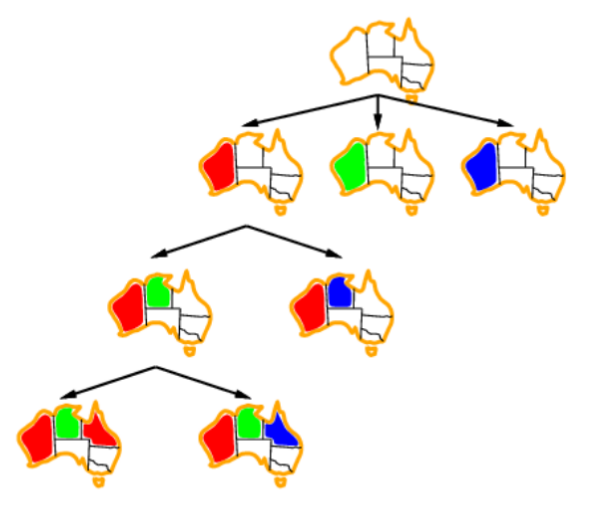
\includegraphics[width=0.5\textwidth]{backtracking}
\end{figure}

\subsection{Euristiche}

Si può scegliere di adottare l'euristica \textbf{minimum remaining values}
(MRV) che consiste nel scegliere di fare branching sulla variabile a cui è
possibile assegnare il minor numero di valori.

Un'altra euristica è la \textbf{most constraining variable} che sceglie la
variabile coinvolta nel maggior numero possibile di vincoli con le altre variabili.

Al contrario, l'euristica \textbf{least constraining value} sceglie la
variabile coinvolta nel minor numero possibile di vincoli con le altre variabili.


